\documentclass{report}
%
% Demo of the mcode package from 
% http://www.mathworks.co.uk/matlabcentral/fileexchange/8015-m-code-latex-package
% Updated 06 Mar 2014
%

% load package with ``framed'' and ``numbered'' option.
\usepackage[framed,numbered,autolinebreaks,useliterate]{mcode}
\usepackage{graphicx}
\usepackage{caption}
\usepackage{subcaption}
\usepackage{wrapfig}
\usepackage{mathtools}
\usepackage{tcolorbox}
\usepackage{parskip}
\usepackage{amssymb}
\usepackage[a4paper, total={6in, 8in}]{geometry}
\geometry{margin=0.7in}
% something NOT relevant to the usage of the package.
\usepackage{url}
\setlength{\parindent}{0pt}
\setlength{\parskip}{10pt}
\title{\texttt{ Regularization for Least Squares Problems}}
\author{Jonathon D'Arcy, \texttt{s1607860}}
% //////////////////////////////////////////////////

\begin{document}
\setlength{\parindent}{25pt}
\maketitle

\clearpage
\noindent A)
\newline \indent In this question, we want to implement the least squares method in Matlab to fit a polynomial to a
set of data observations, these polynomials will be of degree n, for n=1,...,10. We then wish to compute the condition number of $A^{T}A$ in the 2-norm to see the upper bound on its relative error.
\newline


\begin{tcolorbox}
\begin{lstlisting}
load('data_points_50.mat')
A=ones(50,1);
for k=2:11
    A=[A a.^(k-1)];
    x=b\A;
    x = [zeros(1,11-k),x];
    disp(sprintf('p(x) = %3.3fx^10 + %3.3fx^9 + %3.3fx^8 + %3.3fx^7 + %3.3fx^6 + %3.3fx^5 + %3.3fx^4 + %3.3fx^3 + %3.3fx^2 + %3.3fx + %3.3f',x))
    condition=cond(A'*A,2);
    disp(sprintf('The condition number of the %d degree polynomial is %3.2f',k-1,condition));
end
\end{lstlisting}

\begin{center}
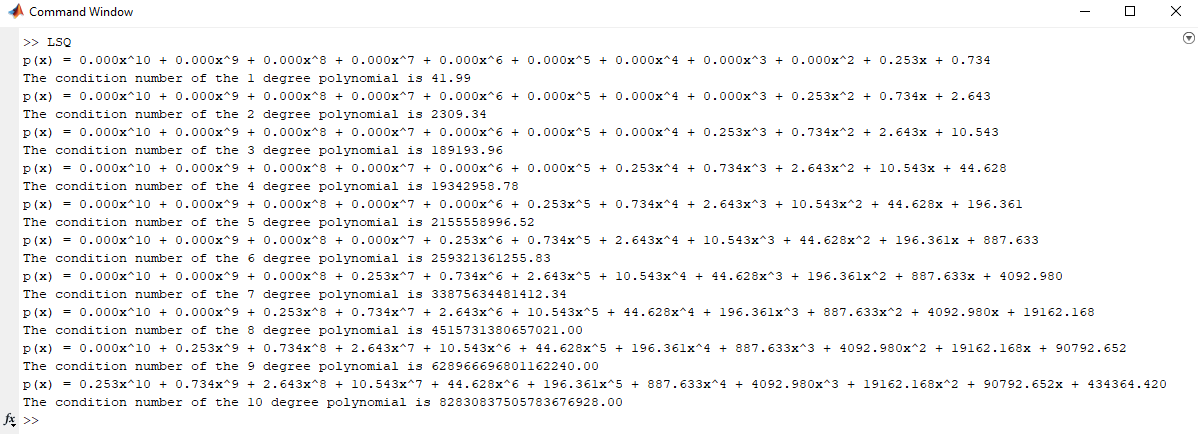
\includegraphics[width=\textwidth] {LSQ_Output_1.png}
\end{center}
\end{tcolorbox}
\vspace{1cm}

\begin{wrapfigure}{l}{0.5\textwidth}
    \centering
    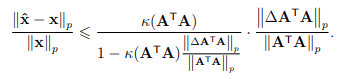
\includegraphics[width=0.5\textwidth]{Error_thrm.png}
\end{wrapfigure} 
\noindent We can clearly see that the Condition numbers of A\textsuperscript{T}A in the Euclidean Norm become very large as we increase the size of our Vandermonde Matrix. This tells us that we have a very large relative error bound on x, as described by the adjacent theorem. In response to this we should try and avoid the form of A\textsuperscript{T}A and attempt to create the reduced form of the Singular Value Decomposition of A, in which we exploit the fact that the diagonal matrix $\Sigma$ will have m-n rows which are zero, and thus we only have to work with certain columns of U. Doing this allows us to avoid $\kappa$(A\textsuperscript{T}A) and instead work directly with $\kappa$(A).
 
\clearpage
\noindent B)
\newline
\setlength{\parindent}{25pt}
\indent From the previous problem we can see the matrix $A^TA$ is badly condition so to avoid having such a large error bound we can compute and use the reduced singular value decomposition of A instead. It should be noted here that the code used to create the graphs for part Ci is contained also in this code and the method for calculating the Average error for each polynomial based off of the same method displayed in this code but is omitted for space, this is attached along with submission however under LSQ\_SVD\_error.m

\begin{tcolorbox}
\begin{lstlisting}
load('data_points_50.mat')
A=ones(50,1);
C = {'k','r','g','y','c','m',[0.2,0.5,0.4],
[0.7,0.7,0.3],[0.7,0.3,0.7],[0.3,0.7,0.7]};
plot(a, b, 'bo', 'LineWidth',2);
for k=2:11
    hold on
    A=[A a.^(k-1)];
    [U,S,V] = svd(A);
    L = length(find(diag(S)));
    U_1=U(:,1:L);
    S_1 = S(1:L,1:L);
    y = S_1\(U_1'*b);
    c = flipud(V*y);
    x = [zeros(11-k,1);c];
    a_space = linspace(0,7,150);
    b_space = x(1)*a_space.^10+x(2)*a_space.^9+x(3)*a_space.^8+
            x(4)*a_space.^7+x(5)*a_space.^6+x(6)*a_space.^5+
            x(7)*a_space.^4+x(8)*a_space.^3+x(9)*a_space.^2+
            x(10)*a_space+x(11);
    plot(a_space, b_space,'color',C{k-1},'LineWidth', 2);
    disp(sprintf('Fitting with the %d degree polynomial',k-1));
    disp(sprintf('p(x) = %3.3fx^10 + %3.3fx^9 + %3.3fx^8 + %3.3fx^7 + %3.3fx^6 + %3.3fx^5 + %3.3fx^4 + %3.3fx^3 + %3.3fx^2 + %3.3fx + %3.3f',x))
    hold off
end
axis([0 7 -5 15])
xlabel('a','FontSize',12)
ylabel('b','FontSize',12)
title('K degree Polynomial fitting amoung data')
legend({'Data','Linear fit','Degree 2 fit','Degree 3 fit','Degree 4 fit','Degree 5 fit','Degree 6 fit','Degree 7 fit','Degree 8 fit','Degree 9 fit','Degree 10 fit'},'Location','NorthWest','NumColumns',2);
\end{lstlisting}
\begin{center}
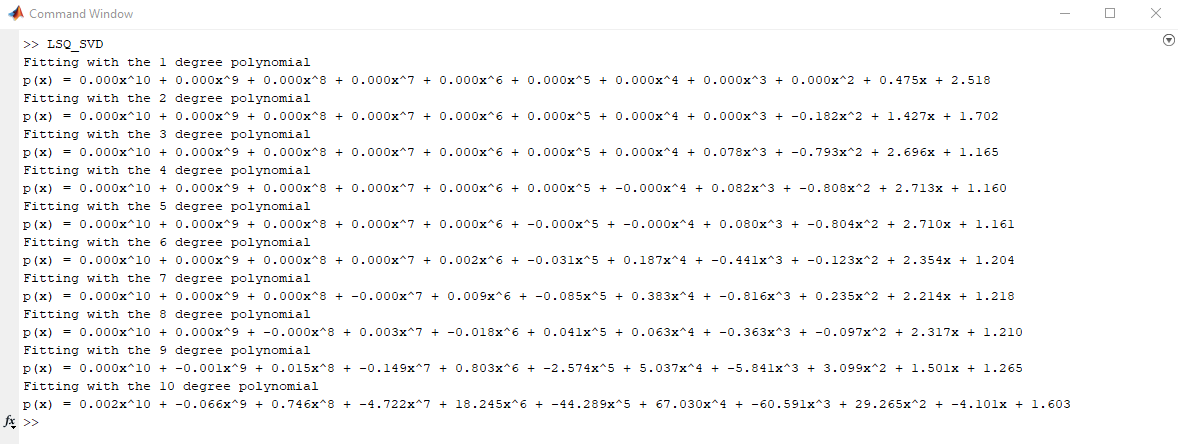
\includegraphics[width=\textwidth] {LSQ_SVD_Output.png}
\end{center}
\end{tcolorbox}
\clearpage
\noindent C)i)
\begin{tcolorbox} 
\begin{center}
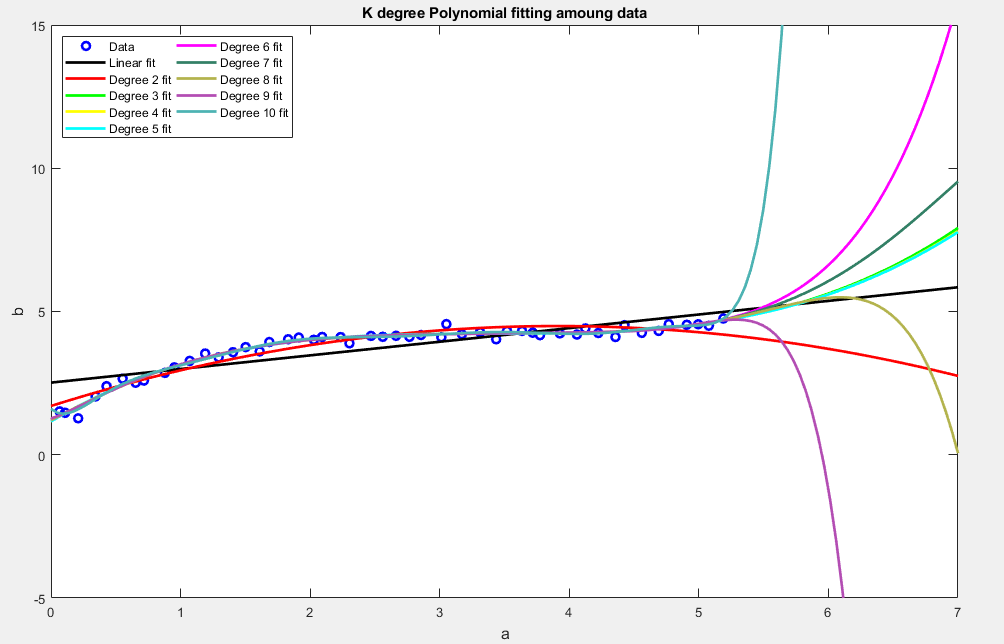
\includegraphics[width=\textwidth] {LSQ_SVD_Graph.png}
\end{center}
\end{tcolorbox}
\begin{tcolorbox}
\begin{center}
     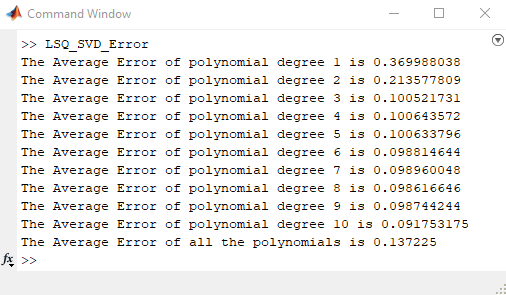
\includegraphics[width=\textwidth]{Poly_test.png}
\end{center}
\end{tcolorbox}The graphs of the polynomials when plotted against the data gives rise to a few interesting observations. Firstly, that when strictly observing the interpolation of our polynomials we appear see a decrease in error as we increase the order of our polynomials. In other words on the domain of our data the higher the degree of the polynomial the closer it relates to the data. This observation is easily testable by averaging the absolute difference of every data point and it's approximated linear regression point, the results of this test is displayed in the output of file LSQ\_SVD\_Error.m and we see that on a whole this tend is true, as were increasing the order of our polynomials we are decreasing the error, however this is not a monotonic principle, take the polynomials of degree 9 and 8 for example, here we see that the 8th degree polynomials has less error than the 9th degree polynomial. The second observation we make comes from the extrapolation of our polynomials, or in other words how they appear to predict the data outside the domain on the original data and by observation of the graph we can see that the larger polynomials tend to predict radical and unexpected changes while lower polynomials tend to stay in line with what expected further data may give. This issue is due to the problem of overfitting, which is when the analysis of data corresponds too closely or exactly to a particular set of data, causing it to fail to fit additional data or predict future observations. In order to combat this we can impliment regularization and for the case of this project, Tikhonov regularization. 
\newline
\newline
\newline
\newline
\noindent C(ii)
\newline
Show that if x minimizes $\| Ax-b \|_2^2 + \mu \| x \|_2^2$ , then it solves the regularized normal
equations $(A^TA + \mu I) x = A^Tb$
\newtheorem{problem}{C(ii)}
\begin{equation}
  G(x) = \| Ax-b \|_2^2 + \mu \| x \|_2^2
\end{equation}
Since we are looking for the minimizer of G(x) we want the gradient of G(x) to equal zero.
\begin{equation}
  \nabla G(x) = \nabla (\| Ax-b \|_2^2 + \mu \| x \|_2^2) = 0 \end{equation}
  \begin{equation}
  \nabla G(x) = \nabla ((Ax-b)^T(Ax-b) + \mu x^Tx) = 0 \end{equation}
  \begin{equation}
  \nabla G(x) = \nabla (x^TA^TAx-2b^TAx+b^Tb + \mu x^Tx) = 0 \end{equation}
  \begin{equation}
  \nabla G(x) =  2A^TAx-2A^Tb + 2\mu x = 0 \end{equation}
    \begin{equation}
  A^TAx + \mu x = A^Tb
\end{equation}
 \begin{equation}
  (A^TA + \mu I) x = A^Tb
\end{equation}
\setcounter{equation}{0}
\newline
\newline
\newline
\newline
\noindent C(iii)
\newline
Let $A=U_1\Sigma_1V^T$ be the reduced SVD of A. Show that x is given by $x = (VSU_1^T)b$ where $S \in \mathbb{R}^{n\times n}$ given by $S_{ii}=\frac{\sigma_i}{\sigma_i^2+\mu}$, for $i=1,...,n$ where $\sigma_i$ is the singular values of A.
\newtheorem{problem_2}{C(iii)}
 \begin{equation}
  (A^TA + \mu I)x = A^Tb
\end{equation}
As we know $A^{T}=V^T\Sigma_1^TU_1^{T}$ and we know $V^T$ $\Sigma_1^T$ and $U_1^{T}$ are all invertable we know that $A^{T}$ is also invertable
 \begin{equation}
 A^{-T}((A^TA + \mu I)x) = b
\end{equation}
\begin{equation}
 (A^{-T}A^TA + A^{-T}\mu I)x = b
\end{equation}
\begin{equation}
 (A + (U_1\Sigma_1 V^T)^{-T}\mu I)x = b
\end{equation}
\begin{equation}
 (U_1\Sigma_1 V^T + U_1^{-T}\Sigma_1^{-T} V^{-1}\mu I)x = b
\end{equation}
Since $U_1$ and $V$ are Orthogonal we can reduce to
\begin{equation}
 (U_1\Sigma_1 V^T + U_1\Sigma_1^{-T} V^T\mu I)x = b
\end{equation}
And since $\mu$ is a constant and I is the Identity matrix it doesn't matter where we multiply them in as long as they stay within the chain of multiples they are in so we can rewrite this as 
\begin{equation}
 (U_1\Sigma_1 V^T + U_1\Sigma_1^{-T}\mu I V^T)x = b
\end{equation}
Then by the Distributive Property of Matrices
\begin{equation}
 U_1(\Sigma_1 + \Sigma_1^{-T}\mu I)V^Tx = b
\end{equation}
\begin{equation}
 x = (U_1(\Sigma_1 + \Sigma_1^{-T}\mu I)V^T)^{-1}b
\end{equation}
\begin{equation}
 x = (V^{-T}(\Sigma_1 + \Sigma_1^{-T}\mu I)^{-1}U_1^{-1})b
\end{equation}
\begin{equation}
 x = (V(\Sigma_1 + \Sigma_1^{-T}\mu I)^{-1}U_1^T)b
\end{equation}
If we define $S=(\Sigma_1 + \Sigma_1^{-T}\mu I)^{-1}$ we get the desired format
\begin{equation}
    x = (VSU_1^T)b
\end{equation}
And observing S we see that since $\Sigma_1$ is a diagonal matrix and by definition has no diagonal value $\sigma_{ii}=0$ that S must take form
\begin{equation}
    S^{-1}=\begin{bmatrix}
    \sigma_{11} & 0 &  \dots  & 0 \\
    0 & \sigma_{22} & \dots  & 0 \\
    \vdots & \vdots & \ddots & \vdots \\
    0 & 0 & \dots  & \sigma_{ii}
\end{bmatrix} + \begin{bmatrix}
    1/\sigma_{11} & 0 &  \dots  & 0 \\
    0 & 1/\sigma_{22} & \dots  & 0 \\
    \vdots & \vdots  & \ddots & \vdots \\
    0 & 0 & \dots  & 1/\sigma_{ii}
\end{bmatrix}\mu I
\end{equation}
\begin{equation}
    S^{-1}=\begin{bmatrix}
    \mu\sigma_{11}/\sigma_{11} & 0  & \dots  & 0 \\
    0 & \mu\sigma_{22}/\sigma_{22}  & \dots  & 0 \\
    \vdots & \vdots & \ddots & \vdots \\
    0 & 0 & \dots  & \mu\sigma_{ii}/\sigma_{ii}
\end{bmatrix}
\end{equation}
Thus since $\mu>0$ we have
\begin{equation}
    S=\begin{bmatrix}
   \sigma_{11}/ \mu\sigma_{11} & 0 & \dots  & 0 \\
    0 & \sigma_{22}/\mu\sigma_{22} & \dots  & 0 \\
    \vdots & \vdots & \ddots & \vdots \\
    0 & 0  & \dots  & \sigma_{ii}/\mu\sigma_{ii}
\end{bmatrix}
\end{equation}
\clearpage
\noindent C(iv)/C(v)
\newline
\indent The following script is an adaption of the previously created LSQ\_reg.m script, in this script however we attempt to use the method of regularization to avoid the problem of overfitting. In order to show regularization we need to choose some $\mu's$ for this problem, we have chosen to view what happens to the polynomials for 4 values of $\mu$, these are $\mu=5,0.5,0.1,0.0001$. The resulting graphical outputs of these will be shown, as well as the calculated average error of the respective $\mu's$ however it has been elected not to display the resulting functions of the polynomials this decision was made as to not bombard the reader with 40 equations, if these are wished to be seen the code is calculating them and running the attached code will display all 40.
\newline
\newline
\newline
\begin{tcolorbox}
\begin{lstlisting}
load('data_points_50.mat')
for F=1:4
        if F==1; 
            M=5;
        elseif F==2;
            M=0.5;
        elseif F==3;
            M=0.01;
        else F==4;
            M=10^-5;
        end
A=ones(50,1);
figure(F);
C = {'k','r','g','y','c','m',[0.2,0.5,0.4],[0.7,0.7,0.3],[0.7,0.3,0.7],[0.3,0.7,0.7]};
plot(a, b, 'bo', 'LineWidth',2);
for k=2:11
    hold on
    A=[A a.^(k-1)];
    [U,S,V] = svd(A);
    L = length(find(diag(S)));
    U_1=U(:,1:L);
    S_1 = S(1:L,1:L);
    for t=1:L
        S_1(t,t)=S_1(t,t)/(S_1(t,t)^2+M);
    end
    c = flipud(V*S_1*U_1'*b);
    x = [zeros(11-k,1);c];
    a_space = linspace(0,7,150);
    b_space = x(1)*a_space.^10+x(2)*a_space.^9+x(3)*a_space.^8+
    x(4)*a_space.^7+x(5)*a_space.^6+x(6)*a_space.^5+
    x(7)*a_space.^4+x(8)*a_space.^3+x(9)*a_space.^2+
    x(10)*a_space+x(11);
    plot(a_space, b_space,'color',C{k-1},'LineWidth', 2);
    disp(sprintf('Fitting with the %d degree polynomial and M=%g',k-1,M));
    disp(sprintf('p(x) = %3.3fx^10 + %3.3fx^9 + %3.3fx^8 + %3.3fx^7 + %3.3fx^6 + %3.3fx^5 + %3.3fx^4 + %3.3fx^3 + %3.3fx^2 + %3.3fx + %3.3f',x))
    hold off
end
axis([0 7 -5 15])
xlabel('a','FontSize',12)
ylabel('b','FontSize',12)
title(['K degree Polynomial fitting amoung data with M=',num2str(M)])
legend({'Data','Linear fit','Degree 2 fit','Degree 3 fit','Degree 4 fit','Degree 5 fit','Degree 6 fit','Degree 7 fit','Degree 8 fit','Degree 9 fit','Degree 10 fit'},'NumColumns',2,'Location','NorthWest');
end
\end{lstlisting}

\end{tcolorbox}

\clearpage
\noindent C(iv)/C(v) (Cont.)
\newline
\newline
\begin{tcolorbox}
     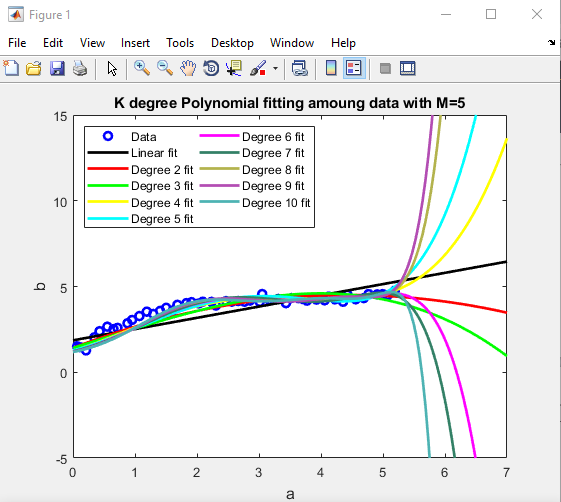
\includegraphics[width=0.5\textwidth]{M=5.png}
      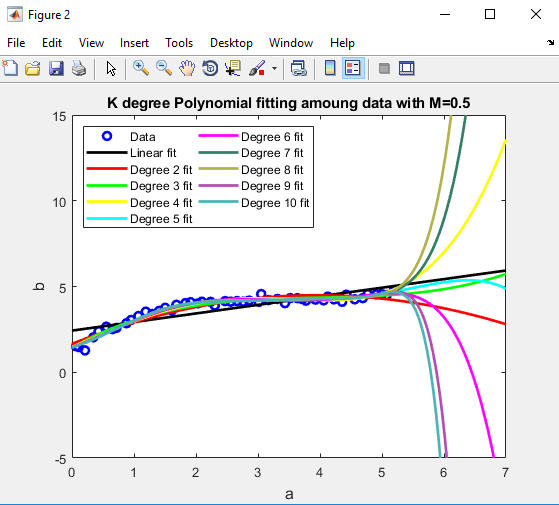
\includegraphics[width=0.5\textwidth]{M=05.png}
       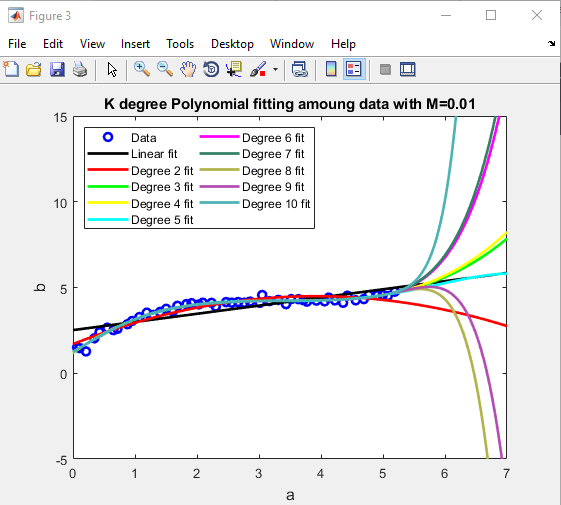
\includegraphics[width=0.5\textwidth]{M=001.png}
        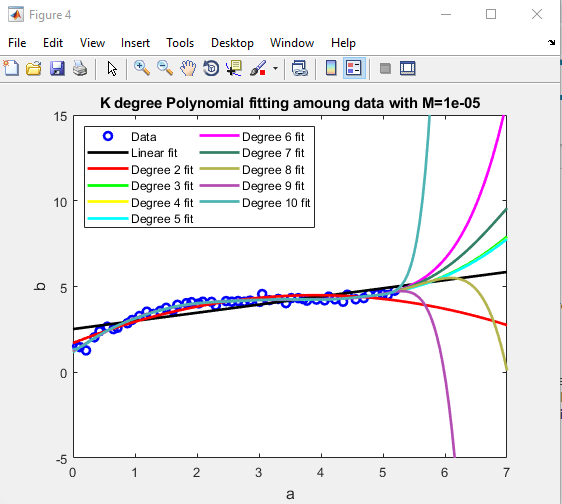
\includegraphics[width=0.5\textwidth]{M=00001.png}
         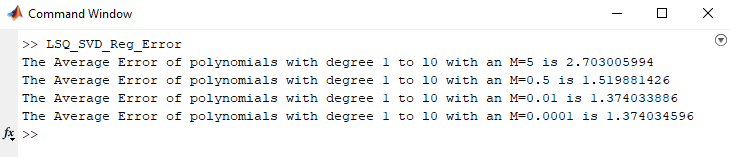
\includegraphics[width=\textwidth]{error_output.png}
\end{tcolorbox}
In the original creations of the polynomials in part B we calculated the average error of each polynomial, if we take the average of those values we get the Average Error of all the polynomials with no regularization, this Average error is 1.372254, comparing this with the Average error of the regularized polynomials we see that adding in regularization increases the error of the polynomials, and that the larger we increase $\mu$ the larger the interpolation error becomes. However we can also notice that if we choose $\mu$ to be too small we are doing very little regularizing and we begin to get very similar plots to the unregulized polynomials. What this all tells us is that if we don't use a large enough regularization we may fall into the problem of over-fitting still, yet if we regularize too much we increase our average error so we need the "Baby-Bear" of $\mu's$, not too large but not too small, for this reason I would say $\mu=0.01$ is the best choice its error is not too far away from the unregularized polynomials and its prediction of data especially of small order polynomials is the closest to the apparent trajectory of the data.

\end{document}
